\section{Deployment}
\label{sec:deploy}

\paragraph{Architecture.}
The public assistant is a static site on GitHub Pages plus a proxy on the Cloudflare Workers free plan, so hosting costs nothing; model calls use the provider's free API tier, so ``zero cost'' holds only within that tier's quotas.
In the browser, a Web Worker embeds the question with bge-small-en-v1.5 (ONNX, half precision, Transformers.js) and searches the structural chunks of all \V{lib.collections} collections (\V{lib.passages} passages from \V{lib.docs} documents), stored as int8 vectors with one scale each (\V{lib.vecgz}\,MB gzip), verified by SHA-256 and kept in the Cache API; passage text is fetched per hit from small shards.
A passage counts as evidence when its cosine reaches its collection's gate threshold (\V{lib.cl.thr} for consumer law and \V{lib.csapp.thr} for CS/AI, a low percentile of the top-1 dev scores of answerable questions; \V{lib.il.thr} for the others).
Packing, citation handling, the guards and the grounded loop are ported to TypeScript, and browser tests check that query embeddings and top results match the Python stack.
The Worker holds the API key, builds every system prompt from the same texts as the Python pipeline, streams replies from \V{wk.model}, and enforces per-visitor limits (\V{wk.per10} requests per ten minutes, \V{wk.perday} per day), a global cap of \V{wk.global} per day and at most \V{wk.maxout} output tokens.

\begin{figure}[t]
\centering
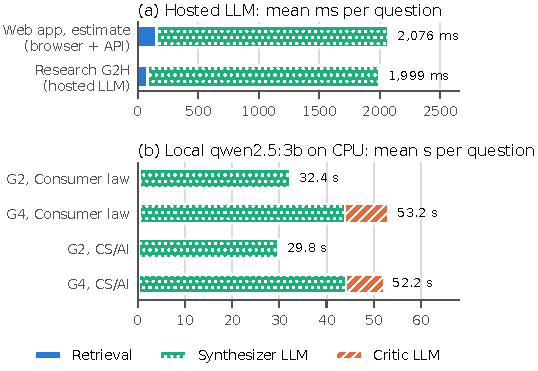
\includegraphics[width=\columnwidth]{figures/latency.pdf}
\caption{Mean latency per question by stage (Table~\ref{tab:generation} reports medians). (a) Hosted generator. The web-app bar is a composed estimate: browser retrieval measured with Playwright on dev questions plus the API latency of the G2H calls; a Grounded-only answer adds at least one critic call, not measured. (b) The local pipeline on the laptop CPU.}
\label{fig:latency}
\end{figure}

\paragraph{Measurements.}
Figure~\ref{fig:latency} and Table~\ref{tab:deploy} (Appendix~\ref{app:tables}) report what we measured on the laptop with headless Chromium and a local static server.
A cold load received \V{web.coldmb}\,MB, almost all of it the embedding model and ONNX Runtime, and was ready after \V{web.cold}\,s; a warm load from the Cache API took \V{web.warm}\,s. These figures exclude network transfer, which dominates a first visit on a real connection; we did not measure the live site over a network.
Per question, embedding took \V{web.embed.p50}\,ms and the search over all indexes \V{web.search.p50}\,ms (medians over \V{web.nq} dev questions); the hosted model call has a median API latency of \V{h.apip50}\,ms (95th percentile \V{h.apip95}\,ms) over the \V{h.calls} G2H calls.
The local pipeline is an order of magnitude slower, mostly in generation.
Lighthouse (mobile) scores the site \V{lh.perf} for performance and \V{lh.a11y}, \V{lh.bp} and \V{lh.seo} for accessibility, best practices and SEO; these page-load scores do not reflect the model download, which starts after the page has loaded.

\paragraph{Privacy.}
Retrieval, uploaded PDFs and conversation history stay in the browser. The question, recent conversation and selected passages go through the Worker to the model provider. Neither the site nor the Worker stores or logs message contents, and the Worker keeps only request times per client address for its rate limits, for at most a day; the provider's handling of the data is governed by its own policy.

\paragraph{Differences from the evaluated pipeline.}
No answer-quality number in this paper measures the public app:
(i) its retrieval is int8 dense bge-small over all collections with a gate, without BM25, fusion, reranking or cross-reference expansion;
(ii) its CS/AI index adds two Python books, and three collections are unevaluated;
(iii) its generator (gpt-oss-120b, budgets \V{web.budget}/\V{web.revbudget}) was evaluated only without guards and critic;
(iv) its ``verified'' stamp comes from the guards and critic, not the NLI judge; and
(v) the gate's abstention and Chat mode were not evaluated.
